\chapter{Implementierung}
In diesem Kapitel sollen ausgewählte Aspekte des zuvor definierten Systems dargelegt werden.
Eingesetzte Technologien und verwendete Werkzeuge, sowie selbst erstellte und externe Bibliotheken werden anhand kurzer Beispiele vorgestellt und deren Funktionsweise aufgezeigt.
Dabei wird auf Probleme, die bei der Entwicklung des Prototypen aufgetreten sind und deren Lösungsansätze eingegangen.

% #####################################################
% ################## Projektstruktur ##################
% #####################################################
\section{Projektstruktur}
Die Projektstruktur wurde in Anlehnung an das PHP Framework Codeigniter\footnote{\url{http://ellislab.com/codeigniter}} angelegt.
Selbiges arbeitet ebenfalls mit dem \ac{MVC} Pattern und legt die einzelnen Komponenten in separaten Ordner an.
Diese wurden auch in Cloudgrid mit \frqq controller\flqq , \frqq models\flqq\ und \frqq views\flqq\ bezeichnet, sodass es dem Entwickler leichter fällt, sich in das Konzept des Systems einzuarbeiten.
Weiterhin wurden die Dateien zur Lokalisierung, genau wie bei Codeigniter, in einem speziellen Ordner abgelegt, der \frqq languages\flqq\ heißt.

\begin{itemize}
    \item CloudGrid/
    \begin{itemize}
        \item controller/
        \item languages/
        \item libraries/
        \item models/
        \item node\_modules/
        \item provider/
        \item public/
        \begin{itemize}
            \item images/
            \item javascripts/
            \item stylesheets/
        \end{itemize}
        \item views/
        \item CloudGrid.js
        \item makefile
        \item package.json
    \end{itemize}
\end{itemize}

Dateien die sich im Ordner \frqq public\flqq\ und deren Unterordner \frqq images\flqq , \frqq javascripts\flqq\ und \frqq stylesheets\flqq\ befinden, dienen zur Einbindung in den Webserver.
Diese Struktur legt das Node.js Framework express nahe, sodass diese auch in CloudGrid übernommen wurde.
Wohingegen der Ordner \frqq node\_modules\flqq\ automatisch von Node.js angelegt wird.
Selbiger beinhaltet Module von Drittanbietern, welche in dem entwickelten Prototypen verwendet werden.
Jegliche selbst entwickelte Module und Bibliotheken werden in dem Ordner \frqq libraries\flqq\ abgelegt.
Lediglich die Module zur Implementierung der Cloudservices wurden in den Ordner \frqq provider\flqq\ ausgelagert.

Im root Ordner \frqq CloudGrid\flqq\ befinden sich drei weitere Dateien.
Das \frqq makefile\flqq\ dient zum Installieren, Deinstallieren und initialen Konfigurieren der Anwendung.
Die Datei \frqq CloudGrid.js\flqq\ dient zum Starten der Anwendung und ist vergleichbar mit der main-Datei einer C-Anwendung.
Um ein Node.js Modul zu erstellen, wird eine \frqq package.json\flqq\ Datei benötigt.
Diese ist zur Ausführung des Programms nicht notwendig, beinhaltet jedoch nützliche Informationen, wie beispielsweise Angaben zum Autor, Abhängigkeiten zu anderen Modulen, sowie Versionsnummer und Name des Moduls.
In der Praxis dient diese Datei dazu, Module in einem Node.js eigenen Paketmanager, welcher npm Registry\footnote{\url{https://npmjs.org}} genannt wird, anzubieten.
Somit wird diese Datei für eine Veröffentlichung im Paketmanager vorbereitet, ohne jedoch zum Abschluss dieser Arbeit dort veröffentlicht zu sein.

% ####################################################
% ################## externe Module ##################
% ####################################################
\section{Externe Module}
\label{implementierung-externe-module}
Externe Module können in Node.js durch den eigenen Paketmanager npm Registry installiert werden.
Dazu muss in der Konsole des Betriebssystems in den Projektordner der Anwendung navigiert werden und der Befehl \frqq npm install packetname\flqq\ eingegeben werden, wobei \frqq packetname\flqq\ durch den Namen des entsprechenden Modul ersetzt werden muss.
Dieses wird daraufhin in den Ordner \frqq node\_modules\flqq\ abgelegt.
Nach Beendigung der Installation kann dieses im Quellcode durch \frqq require\flqq\ geladen werden.

Die hier aufgeführten Module stehen unter der MIT Lizenz\footnote{\url{http://opensource.org/licenses/MIT}}, mit Ausnahme von dem Modul \frqq sqlite3\flqq, welches unter der BSD Lizenz\footnote{\url{http://opensource.org/licenses/bsd-license.php}} steht.
Diese ermöglicht einerseits die freie Bearbeitung aller Module, sowie die kommerzielle und nichtkommerzielle Verwendung.
Somit gibt es seitens der Lizensierung keine Einschränkungen für CloudGrid.

\paragraph{express:}express ist ein Node.js Framework, das sich an das Ruby Framework Sinatra anlehnt\footnote{\url{http://www.sinatrarb.com}}.
Das Modul bringt eine Reihe von essenziellen Funktionalitäten mit.

So ist es möglich, das Projekt nach dem \ac{MVC} Design Pattern zu strukturieren.
Dazu wurden die gleichnamigen Ordner \frqq models\flqq, \frqq views\flqq\ und \frqq controller\flqq\ angelegt.
In \frqq views\flqq\ liegen ausschließlich \ac{HTML} Seiten, welche zur Erstellung der Präsentationsschicht dienen.
Der Ordner \frqq models\flqq\ enthält sowohl die \ac{JSON} Dateien, als auch die SQLite Datenbank, welche zum Speichern der Benutzerdaten dienen.
Im letzten Ordner \frqq controller\flqq\ liegen, die für die Anwendungslogik des Webservers erstellten Dateien.
Diese verknüpfen die Views mit den Modeldaten und werden durch das erweiterte \ac{URI} Routing von express angesprochen.

Durch das Routing können \ac{URI} Pfade festgelegt werden und explizit an Controller gebunden werden.
Quellcode \ref{fig-implementierung-routing} zeigt einen Ausschnitt des Dropbox Routings auf.

\begin{lstlisting}[label=fig-implementierung-routing,caption=Ausschnitt des Dropbox Routings]
var Dropbox = require( './controller/dropbox' ),
    dropbox = new Dropbox();

app.get( '/dropbox/user',           dropbox.getUserInfo );
app.get( '/dropbox/getUrl',         dropbox.getAuthenticationUrl );
app.get( '/auth/dropbox/authorize', dropbox.authorize );
app.get( '/dropbox/getFolder',      dropbox.getFolder );
\end{lstlisting}

In der Projektstruktur existiert weder ein Ordner \frqq dropbox\flqq\ noch eine Datei namens \frqq getFolder\flqq .
Jedoch wird der Anwendung, durch das Initialisieren des Controllers in Zeile 1 und durch das Binden in Zeile 3 bis 7, das Routing bekanntgegeben.
Die \ac{URL} \frqq /dropbox/getFolder\flqq\ greift demnach auf die Klassenmethode \frqq getFolder\flqq\ zu, sobald der Benutzer diese anwählt.
Dieses Prinzip ermöglicht eine strukturierte Programmierung und zugleich eine bessere Lesbarkeit der \acp{URL} für den Benutzer.

Weiterhin ermöglicht express das Senden von \ac{HTTP} Requests und das Empfangen von \ac{HTTP} Responses, einschließlich derer Formulardaten.
Diese sind für Formulare innerhalb der \ac{GUI} wichtig und dienen im konkreten Fall von CloudGrid dazu, die Benutzereinstellungen zu speichern.
Letztendlich unterscheidet sich dieses Verfahren nicht von der äquivalenten Methodik in PHP oder anderen Webprogrammiersprachen.
Auch das Cookiehandling ähnelt in der Handhabung anderen Sprachen, wird jedoch dank express ebenfalls integriert.

Als weiteren großen Vorteil ist die Verwendung von Templateengines zu nennen.
In CloudGrid wird die Hogan Templateengine verwendet, welche auf die mustache.js Template Syntax aufsetzt.
Der Vorteil für den Entwickler liegt darin, die Seite in kleinere Codebausteine zu unterteilen.
In der Praxis wird dadurch Redundanz von \ac{HTML} Code vermieden und die Seiten sind somit leichter anpassbar und eventuelle Fehler können global auf allen Seiten gleichzeitig behoben werden.
Gerade im Entwicklungsprozess ist dieses Verfahren ein erheblicher Vorteil.
Quellcode \ref{fig-implementierung-hogan} zeigt eine entsprechende Seite auf.
Sowohl der Header der Seite, als auch der Footer werden aus externen Bausteinen geladen und in die Seite eingebunden.
Der Entwickler muss sich demnach nur um den jeweiligen Inhalt kümmern.
Dieser besteht im Beispiel aus einer Überschrift und vier Buttons für die einzelnen Anbieter.
Der Code ist kurz gehalten und dennoch gut lesbar.
\newpage
\lstset{
    language=HTML
}
\begin{lstlisting}[label=fig-implementierung-hogan,caption=Aufbau einer mit Hogan erstellten HTML Seite]
{{> header}}
    <h2>Index</h2>
    <div>
        <button id="connect-box" class="box"></button>
        <button id="connect-skydrive" class="skydrive"></button>
        <button id="connect-dropbox" class="dropbox"></button>
        <button id="connect-google-drive" class="googledrive"></button>
    </div>
{{> footer}}
\end{lstlisting}
\lstset{
    language=JavaScript
}

\paragraph{mime:}\frqq mime\flqq\ ist ein einfaches und kleines, dennoch beachtliches Modul, dass den \ac{MIME} Type einer Datei ermitteln kann.
Momentan erkennt es mehr als 600 Dateitypen und mehr als 800 Dateiendungen, welche durch eine aktive Community auf Github stetig erweitert werden.
Das Modul wird zur Erstellung eines \ac{HTTP} Multipart Bodys benötigt, um Dateien zu den Cloudservices hochzuladen.

\paragraph{sqlite3:}Das Modul \frqq sqlite3\flqq\ ist ein Wrapper zur Implementierung einer SQLite Datenbank in Node.js.
Es wird asynchron ausgeführt, sodass die Anwendung bei zeitintensiven SQL Abfragen nicht blockiert wird.
Besonders dieser Punkt ist bei der Umsetzung von CloudGrid essenziell, da beim Abarbeiten der Dateioperationen weder der Webserver, noch die Ordnerüberwachung in der Ausführung unterbrochen werden darf.
Datenbankzugriffe erfolgen an zwei Stellen im Quellcode umgesetzt.
Einerseits beim Initialisieren der Anwendung, wobei die Datenbank angelegt wird, falls diese noch nicht existiert, und zweitens beim Dateihandling.
Bei letztgenannten wird beim Starten der Anwendung geprüft, ob es Veränderungen am Dateisystem gab.
Sollte dies der Fall sein, werden daraufhin die Hashwerte der Dateien mit denen aus der Datenbank verglichen.
Wenn diese nicht übereinstimmen, werden die entsprechenden Dateioperationen erneut durchgeführt.
Zusätzlich wird nach dem Upload einer Datei, deren die Dateiinformationen in die Datenbank gespeichert.

\paragraph{underscore:}underscore.js ist eine schlanke aber überaus hilfreiche Open Source Funktionssammlung, welche unter der MIT Lizenz steht, die grundlegende JavaScript Hilfsfunktionen nachliefert.
Sie ist an Prototype.js\footnote{\url{http://prototypejs.org}} und Ruby\footnote{\url{http://www.ruby-lang.org/de}} angelehnt, ohne dabei bestehende Frameworks vorauszusetzen oder JavaScript Objekte durch Prototyping zu erweitern.
Gut die Hälfte aller Funktionen beziehen sich auf Arrays und Objekte.
So werden Funktionalitäten wie beispielsweise das Durchlaufen eines Arrays mit \frqq \_.each\flqq\ oder Filtern von Einträgen eines Arrays oder auch Objektes realisiert.
Moderne Browser unterstützen bereits einige dieser Funktionen, sodass in diesem Fall auf selbige zurückgegriffen wird.
Durch die Verwendung der underscore.js eigenen Funktionen wird jedoch eine Abwärtskompatibilität für ältere Browser geschaffen.

\paragraph{watchr:}Node.js ist bereits mit einer eigenen Dateisystemüberwachung ausgestattet.
Jedoch weist diese einige Probleme auf.
So wird dieses Modul von Node.js selbst als "`unstable"' bezeichnet, was bedeutet, dass dieses Modul nicht zwingend abwärtskompatibel ist und die durchgeführten Test nicht für eine stabile Version ausreichen.
Darüber hinaus ist kein rekursives Überprüfen von Unterordnern möglich.

Abhilfe schafft da das Modul \frqq watchr\flqq.
Dieses normalisiert die \ac{API} von Node.js, sodass es auch zu früheren Version abwärtskompatibel ist.
Weiterhin ermöglicht es das rekursive Überwachen von Dateien und Ordnern, was für CloudGrid unabdingbar ist.
Aktuell gibt das Modul beim Anlegen, Bearbeiten und Löschen einer Datei oder eines Ordners detaillierte Informationen an den Entwickler zurück.
Dieser kann das entsprechende Event entgegennehmen und darauf reagieren.
In einer zukünftigen Version wird auch das Event \frqq umbenennen\flqq\ integriert, welches momentan nur mit einem Workaround realisierbar ist.
\frqq watchr\flqq\ ist ein wichtiger Bestandteil der Anwendungslogik und deckt die Anforderungen für CloudGrid weitestgehend ab.

% ########################################################################################
% ################## selbst entwickelte Klassen und Funktionssammlungen ##################
% ########################################################################################
\section{Selbst entwickelte Klassen und Funktionssammlungen}
\label{implementierung-self-dev-classes}
In diesem Abschnitt wird auf die relevanten selbst entwickelten Klassen und Funktionssammlungen eingegangen.
Dabei soll deren grobe Funktionsweise und Anwendungsgebiet aufgezeigt werden.

\paragraph{filehelper:}
Der \frqq filehelper\flqq\ ist eine Funktionssammlung, welche Methoden für Dateioperationen beinhaltet, unter anderem jene, die vor dem Upload einer Datei auf selbige anzuwenden sind.
Dazu zählt das Komprimieren, Verschlüsseln und Splitten einer Datei, sowie deren Umkehrung, also das Dekomprimieren, Entschlüsseln und Zusammenfügen.
Weiterhin existieren Funktionen, welche es ermöglichen, alle Dateien eines Ordners zu löschen und ein Array von Dateien zu löschen.
Erstgenannte wird benötigt, um den Temp-Ordner beim Start der Anwendung zu leeren.
Letztere löscht alle temporär erstellten Dateien nach dem Upload einer Datei.
Nicht zuletzt wurde eine Funktion entwickelt, welche die Checksumme einer Datei zurück gibt.
Diese wird in CloudGrid in die Datenbank gespeichert und nach dem Download einer Datei verglichen, um sicherzustellen, dass die Datei konsistent ist.

\paragraph{infologger:}
Die Klasse \frqq infologger\flqq\ dient zum Speichern von Ereignissen während der Ausführung von CloudGrid.
Dazu wird im versteckten Ordner \frqq .logging\flqq\ für jeden Tag eine Datei angelegt, in der Informationen gespeichert werden.
Der Benutzer hat in der \ac{GUI} die Möglichkeit, sich die Einträge der Datei ausgeben zu lassen.
Es gibt drei Methoden, \frqq log\flqq\ , \frqq error\flqq\ und \frqq warning\flqq , zum Schreiben von Einträgen.
Hierbei wendet der Programmierer, je nach Ereignis, die entsprechende Methode an.
Alle Einträge beginnen mit einem Datum, gefolgt von einer Tilde und dem entsprechenden Text.
Sollte die Methode error verwendet werden, wird dem Text das Wort \frqq error:\flqq\ vorangestellt und bei warning das Wort \frqq warning:\flqq .
Diese Klasse wird global in CloudGrid eingebunden, sodass diese in allen Modulen verfügbar ist und verwendet werden kann.

\paragraph{initialize:}Beim Starten von CloudGrid müssen diverse Funktionen ausgeführt werden, welche die Konsistenz der Daten sicherstellen.
Beispielsweise wird der \frqq temp\flqq\ Ordner geleert, sodass nicht unnötig Speicherplatz belegt wird.
Die \ac{JSON} Konfigurationsdateien werden auf ihre Existenz geprüft und im Falle eines Nichtvorhandenseins neu angelegt, genau wie die SQLite Datenbank.
Darüber hinaus wurden Funktionen erstellt, welche beim ersten Start der Anwendung direkt nach der Installation zum initialen Setup dienen.
Außerdem befinden sich die Methoden zum Überprüfen des Dateisystems auf Veränderungen seit dem letzten Ausführen der Anwendung, sowie der Überprüfung der Dateien auf den Cloudservices in der Klasse.
Dementsprechend braucht die Klasse relativ viel Zeit zum Ausführen, was die erste Nutzung der Anwendung verzögert.
Dieser Aspekt bedarf einer Optimierung und sollte in zukünftigen Versionen angepasst werden.

\paragraph{multipart:}
Die \frqq multipart\flqq\ Klasse dient zum Erstellen von \ac{HTTP} Multipart Bodies.\footnote{\url{http://www.w3.org/TR/html4/interact/forms.html\#h-17.13.4.2}}
Diese werden unter anderem beim Upload von Dateien benötigt.
Quellcode \ref{fig-implementierung-multipart} zeigt beispielhaft einen solchen auf.

Ein Multipart Body wird in mehrere Abschnitte unterteilt.
Einerseits muss ein entsprechender \ac{HTTP} Body an den Server mitgegeben werden, damit dieser den Request entsprechend abarbeiten kann, andererseits müssen die entsprechenden Daten übergeben werden.
Diese können wiederum im Klartext oder als Binärdaten übergeben werden.
Letzteres dient dabei der Übertragung von Dateien an einen Server.
Alle Fomularfelder durch einen eindeutigen Schlüssel, der Boundary heißt, von einander getrennt.
Dies ist ein eindeutiger Schlüssel, der die einzelnen Abschnitte untergliedern soll.
Hierbei ist die Eindeutigkeit des Schlüssels ein zwingendes Kriterium.
Sollte dieser im Datenbereich eines Formularfeldes auftreten, kann der ganze Multipart Body ungültig werden.

\lstset{
    language=PHP
}
\begin{lstlisting}[label=fig-implementierung-multipart,caption=Beispiel eines HTTP Multipart Bodies]
POST /path/to/script.php HTTP/1.0
Host: example.com
Content-type: multipart/form-data, boundary=AaB03x
Content-Length: body_length

--AaB03x
content-disposition: form-data; name="field1"

Test Daten
--AaB03x
content-disposition: form-data; name="userfile"; filename="$filename"
Content-Type: application/pdf
Content-Transfer-Encoding: binary

binäre Daten
--AaB03x--
\end{lstlisting}
\lstset{
    language=JavaScript
}

Die selbsterstellte Bibliothek \frqq multipart\flqq\ greift darüber hinaus auf die externe Bibliothek namens \frqq mime\flqq\ zu, welche es erlaubt, den \ac{MIME} Type einer Datei programmatisch zu bestimmen, um somit den Content-Type Header zu befüllen.
\frqq multipart\flqq\ wird nach Beendigung dieser Arbeit als Open-Source Module in den Node.js eigenen Paketmanager npm eingepflegt, da zum Zeitpunkt der Erstellung dieser Arbeit keine vergleichbaren Module existierten oder deren Lösungen als unzureichend erachtet wurden.

\paragraph{oauth2:}
Die oauth2 Klasse basiert auf einem Node.js Modul Namens \frqq oauth\flqq \footnote{\url{https://npmjs.org/package/oauth}}.
Dieses steht unter der MIT Lizenz, sodass es möglich war, diese nach Belieben anzupassen.
Grundlegend dient das Modul dazu generelle Aufgaben bei der Verwendung von OAuth2 abzudecken.
Unter anderem kann der Authentifizierungstoken von einem Anbieter abgerufen werden und POST und GET Requests an diesen geschickt werden.
Das Modul hat bereits viele Anforderungen abgedeckt, jedoch war es für die Umsetzung des Prototypen nicht ausreichend, sodass dieses noch um weitere Funktionalitäten erweitert werden musste.
So ist es nun möglich neben POST und GET Request auch DELETE und PUT Request zu erstellen.
Dies ist beispielsweise für die Anbieter Dropbox und Box zwingend notwendig, da diese Anbieter beide Methoden in ihrer \ac{API} integriert haben.

Weiterhin wurde der Prozess zum Erstellen des Request Bodys angepasst, sodass auch ein Node.js Buffer oder gar ein Array von Buffern anstelle eines Strings an den Body übergeben werden kann und in den entsprechenden Body geschrieben wird.
Neben diesen Anpassungen wurde zudem der Code refactored, was bedeutet, dass einige syntaktische Fehler behoben wurden und der Quellcode besser strukturiert wurde, was die Lesbarkeit erheblich steigert.
Bei diesem Prozess wurden auch mehrere kleinere Fehler ausfindig gemacht, welche zugleich beseitigt wurden.
In Anschluss an diese Arbeit wird auch dieses Modul, genau wie das \frqq multipart\flqq\ Module als Open-Source Module in das npm eingepflegt.

\paragraph{queue:}
\frqq queue\flqq\ ist eine Hilfsklasse, welche es ermöglicht, lang andauernde Funktionen nacheinander auszuführen.
Besonders bei der Verwendung der SQLite Datenbank ist dieses unerlässlich, da diese nur einen Schreibzugriff zur gleichen Zeit zulässt.
Das bedeutet beispielsweise, wenn die Teilstücken einer Datei zu den Cloudservices hochgeladen wurden und die Information darüber in die Datenbank geschrieben werden soll, muss sichergestellt werden, dass die Schreibzugriff nacheinander ausgeführt werden.
Sonst würde das Programm mit einer Fehlermeldung abstürzen.

Die Klasse selbst lehnt sich an dem \frqq reference counting\flqq\ Prinzip an.
Dieses besagt, dass eine Queue, also eine Warteschlange, erstellt und bei jedem Eintrag der hinzugefügt wird, ein klasseninterner Zähler inkrementiert und beim Entfernen eines Eintrages aus der Queue, der Zähler dekrementiert wird.
Solange wie der Zähler nicht auf 0 hinuntergeht, wird die Klasse weiter ausgeführt.
Sollte er auf Null stehen, so wird auf weitere Einträge gewartet.

Um dieses Prinzip umzusetzen, wird ein Array verwendet, welches die einzelnen Funktionen der Queue beinhaltet.
Mit der Methode \frqq push\flqq\ kann ein weiteres Element der Queue hinzugefügt werden.
Ein boolscher Parameter \frqq inProgress\flqq\ gibt an, ob zum Zeitpunkt des Hinzufügens eine Funktion ausgeführt wird oder ob direkt mit der Ausführung der aktuellen Funktion begonnen werden kann.
Sollte keine Funktion ausgeführt werden, so wird die Methode \frqq next\flqq\ aufgerufen.
Diese setzt den Parameter inProgress auf true und nimmt sich daraufhin den obersten Eintrag des Arrays und führt die Funktion aus.
Sollte kein Eintrag mehr im Array existieren, also nach dem Prinzip des \frqq reference counting\flqq\ der Zähler auf Null stehen, so wird der inProgress auf false gesetzt.

Eine Funktion, die an die queue Klasse übergeben wird, muss als Callback die next Methode aufrufen, damit die Funktionalität der Klasse gewährleistet werden kann.
Diese Limitierung ist speziell auf die Verwendung von Node.js zugeschnitten und ist ein gewünschtes Verhalten.
Sollte der Programmierer diese Methodik nicht implementieren, so wird die Queue nicht weiter abgearbeitet.
Im Falle eines Fehlers bei der Ausführung einer Datei, wird dieser abgefangen und die nächste Funktion aufgerufen.

\paragraph{randomhelper:}Eine weitere unterstützende Funktionssammlung ist der \frqq randomhelper\flqq .
Dieser ermöglicht es, verschiedene pseudozufällige Werte zu erzeugen.
So wird beispielsweise die Methode \frqq generateFileName\flqq\ verwendet, um pseudozufällige Dateinamen für die Teilstücke einer Datei zu generieren.
Die Methode \frqq generatePassphrase\flqq\ dient hingegen dazu, einen Passphrase zur Ver- und Entschlüsselung einer Datei zu liefern.

\paragraph{watchrwrapper:}In der Klasse \frqq watchrwrapper\flqq\ wird ein Großteil der Anwendungslogik von CloudGrid umgesetzt.
Alle Dateioperationen werden unter Zuhilfenahme, sowohl der externen Module als auch selbstenwickelter Klassen und Funktionssammlungen, in dieser Klasse umgesetzt.
Zuerst wird das Modul \frqq watchr\flqq\ gestartet, welches in Abschnitt \ref{implementierung-externe-module} bereits vorgestellt wurde.
Dieses überprüft einen, vom Benutzer gewählten Ordner und dessen Unterordner, auf Veränderungen.
Je nach Ereignis wird daraufhin der entsprechende Prozess, \frqq createProcess\flqq , \frqq updateProcess\flqq\ und \frqq deleteProcess\flqq\ genannt, gestartet.
Diese laufen in einer Queue ab, was bedeutet, dass diese synchron nacheinander ausgeführt werden.
Nach Beendigung eines Prozesses wird entweder der nächste gestartet, insofern einer in der Queue existiert, oder die Klasse wartet auf die nächste Veränderung.

\paragraph{provider:}Die Klassen zur Implementierung der einzelnen Cloudservices werden in einem Ordner \frqq provider\flqq\ gespeichert.
Alle Klasse verfügen über einen ähnlichen Funktionsumfang und wurden in Methodenbenennung und Aufbau einheitlich gestaltet.
Lediglich Besonderheiten der einzelnen Provider müssen in den Methoden beachtet werden, was eine einheitliche generische Klasse für alle Anbieter nicht realisierbar macht.
Jede Klasse bekommt im Konstruktor ein Objekt mit Einstellungen übergeben.
Diese werden aus der \frqq provider.json\flqq\ Datei geladen.
Ein späteres Hinzufügen und Auslesen ist durch entsprechende Getter und Setter jedoch ebenfalls möglich.
Weiterhin bindet der Konstruktor die \frqq OAuth2\flqq\ Klasse ein und wird ausgeführt.
Je nach Anbieter wird dann noch geprüft ob ein Access-Token existiert und ob dieser noch gültig ist.
Sollte dem nicht der Fall sein, wird entsprechend mit dem Refresh-Token ein neuer angefordert.
Danach ist die Klasse einsatzbereit.
Alle Methoden werden unter Zuhilfenahme der \frqq oauth2\flqq\ Klasse ausgeführt und entsprechend der Dokumentation des Anbieters umgesetzt.
Jedes Modul wurde wiederverwendbar entwickelt.
In Anschluss an diese Arbeit wird auch bei den Provider Modulen erwägt, diese als Open-Source Module in das npm einzupflegen, da es zum Zeitpunkt der Erstellung dieser Arbeit keine Module für Box, Microsoft Skydrive oder Google Drive existierten.
\newpage
\section{Realisierung der Datenhaltungs-Schicht}
Die physische Datenhaltung wird durch zwei Konzepte realisiert.
Durch die Speicherung einfacher JavaScript Strings in einer \ac{JSON} Datei werden alle Konfigurationseinstellungen gespeichert.
Dazu zählen die Einstellungen zu den Cloudservices, welche exemplarisch im Quellcode \ref{fig-implementierung-provider-json} aufgeführt sind, sowie die Systemeinstellungen und benutzerspezifischen Einstellungen, dazu zählen der überwachte Ordner, die Anwendungssprache und der Port des Webservers.

\begin{lstlisting}[label=fig-implementierung-provider-json,caption=JSON String eines Cloudservices]
{
    "box": {
        "id": 1,
        "client_id": "506o7ezrhhikyx35bwcyuzzg2zxxx",
        "client_secret": "KMWtKieXazyRHtQXzxrOC6JlCIxxx",
        "base_site": "https://www.box.com/",
        "authorize_url": null,
        "access_token_url": "api/oauth2/token",
        "custom_headers": null,
        "access_token": "SAuJtuY7VrBd3ZGj3lPOKaJj7qQxxx",
        "refresh_token": "h2G9BFxcsvpoklapuDTvf0uky0haTAxxx",
        "expires": 1374799440,
        "redirect_uri": "http://127.0.0.1:8080/auth/box/authorize",
        "connected": true
    }
}
\end{lstlisting}

Jegliche \ac{JSON} Dateien werden bei dem Anwendungsstart von der selbst entwickelten Bibliothek \frqq jsonreader\flqq\ eingelesen und in einer globalen Variable vorgehalten.
Diese ist auch in allen Submodulen verfügbar, sodass die Anwendung jederzeit Zugriff auf diese Informationen hat.
Der Vorteil daran ist, dass die Datei lediglich einmal beim Anwendungsstart eingelesen werden muss und nicht jedes Mal, wenn diese benötigt wird.
Sollten sich Daten ändern, so wird die komplette Datei neu geschrieben.
Da Änderungen an den Einstellung selten vorkommen und die zu speichernden Daten einen geringen Umfang haben, ist dieses Verfahren überaus performant.

Bei der Wahl des Formats zum Speichern der Informationen wurde \ac{JSON} gewählt, da es, wie der Name bereits erahnen lässt, von Hause aus in JavaScript implementiert und dementsprechend leicht umsetzbar ist.
Die Daten werden aus der Datei ausgelesen und in ein JavaScript Object umgewandelt.
Danach ist es möglich Attribute, ähnlich wie in einer Klasse, direkt anzusprechen.
Gerade bei verschachtelten Strukturen ist es somit leichter möglich auf Attribute zuzugreifen.

Die zweite verwendete Methode ist die Speicherung der Daten in einer SQLite Datenbank.
Diese hat den Vorteil, dass sie sich direkt in eine Anwendung implementieren lässt und keine weitere Server-Software benötigt wird.
Erforderlich ist lediglich die Einbindung einer entsprechenden Bibliothek.
Im konkreten Fall von CloudGrid wird das \frqq sqlite3\flqq\ Modul verwendet.
Die Datenbank selbst liegt im Ordner \frqq models\flqq\ und heißt config.db.
Diese enthält lediglich zwei Tabellen.
In Abbildung \ref{fig-implementierung-sql} sind diese schematisch aufgezeigt.

\begin{figure}[H]
  \centering
  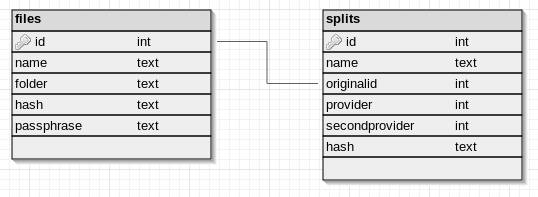
\includegraphics[scale=0.6]{resources/Bilder_Kapitel_5/sql.png}
  \caption{Schema der SQLite Datenbank}
  \label{fig-implementierung-sql}
\end{figure}

Die Tabelle \frqq files\flqq\ speichert Informationen zur Originaldatei, den Namen, den Ordner in dem diese auf dem lokalen Dateisystem gespeichert ist, sowie den Hash des Inhalts und den Passphrase zum Ent- und Verschlüsseln der Datei.
Der Hash wird benötigt um nach dem Download einer Datei und der Durchführung der Dateioperation zu prüfen, ob die Datei korrekt wiederhergestellt wurde.

In Tabelle \frqq splits\flqq\ werden die Informationen zu den Teilstücke einer Datei gespeichert.
Neben dem Namen und der Verknüpfung zur ursprünglichen Datei, hier \frqq originalid\flqq\ genannt, wird ein weiterer Hash gespeichert und die Provider, bei denen die Datei geuploaded wurde.
Der Wert \frqq providerid\flqq\ entspricht der ID aus der \ac{JSON} Datei, welche im Quellcode \ref{fig-implementierung-provider-json} aufgeführt ist.
Somit können programmatisch die Teilstücke von den einzelnen Anbietern geladen werden.
Nachdem der Download beendet ist, werden die Teilstücke mit den in der Datenbank gespeicherten Hashwerten verglichen, um auch in diesem Fall die Dateiintegrität sicherzustellen.

% ##############################################################################
% ################## Realisierung der Anwendungslogik-Schicht ##################
% ##############################################################################
\section{Realisierung der Anwendungslogik-Schicht}
\label{implementierung-realisierung-anwendungslogik}
Der Workflow der Anwendungslogik-Schicht beginnt mit dem Initialisieren der Anwendung.
Hierbei wird als Erstes die Konsistenz der benötigten Ordner überprüft.
Dazu zählen der temp, logging und models Ordner.
Sollte einer dieser drei Ordner nicht existieren, wird er von der Anwendung angelegt.
Daraufhin werden die \ac{JSON} Dateien im models Ordner überprüft.
Sollten auch diese nicht vorhanden sein, werden sie angelegt und mit Standardwerten gefüllt.
Als weiterer Schritt wird geprüft, ob die SQLite Datenbank existiert.
Sofern sich auch diese nicht im models Ordner befindet, wird sie angelegt und die beiden Tabellen erzeugt.
Abschließend wird der temp Ordner geleert, für den Fall, dass sich noch temporäre Dateien in diesem befinden.
Dieser Vorgang wird sowohl beim ersten Starten der Anwendung durchgeführt, als auch bei jedem weiteren Start.
Eine Unterscheidung dieser beiden Vorgänge wird nicht getroffen.

Wenn sich die Daten der Anwendung daraufhin in einem konsistenten Zustand befinden, werden alle Einstellungen geladen.
Die Daten aus den \ac{JSON} Dateien werden gelesen und in einer globale Variable im System hinterlegt.
Das ermöglicht bei der Ausführung von CloudGrid einen schnelleren Zugriff auf diese Daten und vermindert die Anzahl der Zugriffe auf das Dateisystem.

Sobald auch dieser Vorgang abgeschlossen ist, wird parallel der Webserver und die Ordnerüberwachung gestartet.
Auf Seiten des Webservers werden dazu alle Einstellungen geladen, wie beispielsweise der Port, auf dem die Webseite laufen soll, die Templateengine wird festgelegt und die einzelnen Standardtemplates vorgeladen.
Zusätzlich werden alle Routen definiert.
Außerdem werden die gespeicherten OAuth-Token der Cloudservices auf Aktualität geprüft.
Sollte der access token eines Services abgelaufen sein, so wird dieser, mit Hilfe des refresh tokens, erneuert.

Die Initialisierung der Ordnerüberwachung erfolgt in mehreren Schritten.
Als Erstes wird das aktuelle Dateisystem auf Veränderungen überprüft.
Dazu werden, mit der selbsterstellen Klasse \frqq foldertree\flqq , alle Dateien erfasst und deren Hashwert ermittelt, um diese daraufhin mit dem Hashwert in der Datenbank zu vergleichen.
Sollten die diese nicht übereinstimmen, so werden zuerst die Teilstücke der Datei bei den Cloudservices gelöscht, um danach die Dateioperationen auf die Datei anzuwenden und diese anschließend auf die Cloudservices zu verteilen.
Wenn jedoch eine Datei nicht in der Datenbank existiert, so wird diese in die Datenbank aufgenommen, die Dateioperationen angewendet und entsprechend zu den Cloudservices hochgeladen.
Abschließend werden gelöschte Dateien ermittelt, das bedeutet, alle Dateien welche sich in der Datenbank befinden, jedoch nicht auf dem Dateisystem.
Wenn dieser Fall eintritt, werden sowohl die Teilstücke auf den Cloudservices, als auch die Informationen über die Datei aus der Datenbank gelöscht.

Wenn dieser Vorgang beendet ist, wird die Konsistenz der Teilstücke bei den Cloudservices überprüft.
Dazu werden die Informationen zu den Teilstücken aus der Datenbank ausgelesen und selbige auf Existenz bei den Cloudservices geprüft.
Wenn ein Teilstück fehlen sollte, wird versucht dieses bei dem redundanten Cloudservices herunterzuladen und erneut hochzuladen.
Sollte das Teilstück bei allen Cloudservices gelöscht worden sein, so werden alle Teilstücke der originalen Datei auf den Cloudservices gelöscht, sowie die Informationen in der Datenbank, um die Datei daraufhin wie eine Neuanlage zu betrachten und den bereits beschriebenen Vorgang durchzuführen.

Nach der erfolgreichen Durchführung dieses Vorganges wird letztendlich die Ordnerüberwachung gestartet.
Diese überwacht einen vom Benutzer angegebenen Ordner auf Veränderung.
Dabei können die in Abschnitt \ref{systementwurf-dateihandling} beschriebenen Dateioperationen, anlegen, löschen, bearbeiten, umbenennen und verschieben einer Datei, auftreten.
Jeder dieser Fälle muss einzeln abgearbeitet werden.
Um sicherzustellen, dass die einzelnen Funktionen erfolgreich durchgeführt werden können und sich beim Zugriff auf die Datenbank nicht gegenseitig blockieren, werden sie, unter Zuhilfenahme der queue Klasse, in eine Warteschlange eingefügt.
Diese führt alle dort enthaltenden Funktionen nacheinander aus, sodass keine gleichzeitigen Zugriffe auftreten können.

\paragraph{Anlegen:}Beim anlegen einer Datei wird die Methode \frqq createProcess\flqq\ ausgeführt.
Diese prüft zuerst, ob die angegebene Datei wirklich existiert und ob es sich um eine Datei oder einen Ordner handelt.
Sollte die Datei nicht existieren oder ein Ordner übergeben worden sein, so bricht die Methode mit einer Fehlermeldung ab.
Ansonsten beginnt sie mit der Komprimierung der Datei.
Dabei wird eine Funktion aus dem filehelper verwendet.
Zum Komprimieren wird die Node.js eigene \frqq zlib\flqq\ Klasse verwendet.
Eine Datei, die komprimiert wurde, wird in dem temp Ordner der Anwendung gespeichert und mit der Dateiendung \frqq zip\flqq\ versehen.
Sollte dieser Vorgang erfolgreich gewesen sein, so wird ein Passphrase erstellt und die Datei daraufhin verschlüsselt.
Auch in diesem Fall wird die Datei im temp Ordner gespeichert und mit der Dateiendung \frqq crypt\flqq\ versehen.
Nach der erfolgreichen Verschlüsselung wird die Datei gesplittet.
Dazu wird zuerst die Anzahl der eingebundenen Cloudservices ermittelt, um anhand dieser die Anzahl der Teilstücken zu bestimmen.
Beim Splitten wird jedes Teilstück mit einem pseudozufälligen Dateinamen versehen und im temp Ordner gespeichert.
Im Anschluss daran werden die eingebundenen Cloudservices ausgewählt und der Upload der Dateien wird durchgeführt.
Abschließend werden alle Informationen zur originalen Datei und zu den Teilstücken in der SQLite Datenbank gespeichert und alle temporären Dateien aus dem temp Ordner gelöscht.
Sollte in dem gesamten Prozess ein Fehler auftreten, so wird dieser unter Zuhilfenahme der \frqq infologger\flqq\ Funktionssammlung in eine Logging Datei geschrieben und kann vom Benutzer in der \ac{GUI} eingesehen werden.
Der Prozess selbst wird abgebrochen und der nächste Prozess gestartet, insofern es einen weiteren in der Queue gibt.

\paragraph{Löschen:}Beim Löschen einer Datei wird die Methode \frqq deleteProcess\flqq\ ausgeführt.
Diese ermittelt zuerst die Datenbank ID der originalen Datei, um daraufhin alle Teilstücke zu selektieren.
Sobald diese Informationen vorliegen, werden alle Teilstücke bei allen Cloudservices gelöscht.
Dazu werden die entsprechenden Methoden in den Provider Klassen ausgeführt.
Abschließend werden die Einträge in den Datenbanken gelöscht.
Auch die deleteProcess Methode wird durch die infologger Funktionssammlung protokolliert und an die Queue übergeben.

\paragraph{Bearbeiten:}Die Bearbeitung einer Datei ähnelt einer Vereinigung der beiden zuvor vorgestellten Prozesse.
Sollte sich der Inhalt einer Datei verändern, werden zuerst alle Teilstücke einer Datei auf den Cloudservices und zugleich deren Informationen aus der Datenbank gelöscht.
Die Informationen zu der originalen Datei bleiben in der Tabelle files in der Datenbank erhalten.
Daraufhin wird der Hash der Datei neu berechnet und der Datenbankeintrag entsprechend geupdatet.
Anschließend werden die Dateioperationen, welche auch im \frqq createProcess\flqq\ durchgeführt wurden, ausgeführt.
Die Teilstücke werden dann zu den Cloudservices hochgeladen und die Informationen in die Datenbank geschrieben.

\paragraph{Umbenennen/Verschieben:}Zum Zeitpunkt der Erstellung der Arbeit bietet das Modul \frqq watchr\flqq\ keine Methoden zum Erkennen einer Umbenennung oder Verschiebung einer Datei.
Dadurch ergibt sich ein großer Nachteil bei der Implementierung in CloudGrid.
Normalerweise würde lediglich der Dateiname beziehungsweise der Pfad zur Datei in der Datenbank angepasst werden und die Teilstücke einer Datei bei den Cloudservices könnten unverändert bleiben.
Durch das Fehlen der Methode wird das Umbenennen und auch das Verschieben einer Datei als Löschen und anschließend Erstellen einer Datei angesehen.
Das beeinträchtigt erheblich die Effizienz von CloudGrid.
Dieser Umstand muss in einer späteren Version des Prototypen angepasst werden, um unnötige Datei- und Uploadoperationen zu vermeiden und die Effizienz bei der Ausführung der Anwendung zu steigern.

Die Ordnerüberwachung läuft solange eine Internetverbindung besteht.
Vor der Überwachung wird eine Funktion gestartet, welche im Sekundentakt prüft, ob eine Verbindung zum Internet besteht oder nicht.
Sollte diese unterbrochen werden, so wird auch die Ordnerüberwachung gestoppt und die Queue mit den Prozessen geleert.
Dieser Vorgang wird durch die Funktion \frqq hasInternet\flqq\ der \frqq utils\flqq\ Funktionssammlung realisiert.
Um die Überprüfung umzusetzen, wird ein Datenpaket mittels Ping an google.de geschickt.
Sollte ein Datenpaket zurückgeschickt werden, besteht eine Internetverbindung, ansonsten nicht.
Wenn die Verbindung zum Internet wieder aufgebaut wurde, wird automatisch die Ordnerüberwachung gestartet und der zuvor aufgezeigte Vorgang erneut durchgeführt.
Dadurch, dass die initiale Überprüfung der Dateien durchgeführt wird, werden auch Prozesse, die zuvor aus der Queue gelöscht wurden, erneut ausgeführt.

% ###########################################################################
% ################## Realisierung der Präsentationsschicht ##################
% ###########################################################################
\section{Realisierung der Präsentationsschicht}
Die Umsetzung der Präsentationsschicht ist bewusst einfach gehalten.
Zur Gestaltung wurde \ac{CSS} verwendet, welches aus \ac{Sass} Dateien generiert wird.
\ac{Sass} ist eine Scriptsprache, welche eine programmatische Erstellung von \ac{CSS} Dateien ermöglicht.
Insbesondere die Verwendung von Variablen und Funktionen, Mixins genannt, erleichtern die Arbeit mit \ac{CSS} erheblich, wodurch das Stylesheet sich später flexibler anpassen lässt.
Eine \ac{Sass} Datei muss nach der Erstellung kompiliert werden, was der mitgelieferte \ac{Sass}-Compiler realisiert.

Bei der Umsetzung des Designs für die \ac{GUI} werden vier \ac{CSS} Dateien verwendet.
Die \frqq normalize.scss\flqq\ dient dazu, die Voreinstellungen von \ac{HTML} Elementen in verschiedenen Browsern zurückzusetzen.
Hierbei wird das normalize Projekt\footnote{\url{https://github.com/necolas/normalize.css}} verwendet.
Diese steht unter der MIT Lizenz und kann somit frei verwendet werden.

Die zweite Datei \frqq mixins.scss\flqq\ ist eine selbsterstellte Funktionssammlung, welche sich wiederholende Style-Definitionen umsetzt.
Beispielsweise dient das Mixin \frqq clearfix\flqq\ dazu, gefloatete Elemente zu clearen oder das \frqq center-page\flqq\ Mixin, um den Header, Footer und Contentbereich in der Seite zu zentrieren.

Die \frqq variables.scss\flqq\ Datei beinhaltet alle Variablen, welche in den \ac{Sass} Dateien verwendet werden.
Der Vorteil hierbei ist, dass das Farbkonzept der Seite schnell bearbeitet werden kann, da alle Farben in entsprechende Variablen ausgelagert wurden.
So können Themes angelegt werden, ohne das eine komplette \ac{CSS} oder \ac{Sass} Datei refactored werden muss.

Abschließend existiert noch die \frqq main.scss\flqq\ .
Diese beinhaltet alle Styleangaben für die einzelnen Elemente der Webseite.
Jede der zuvor genannten Dateien wird am Anfang der \frqq main.scss\flqq\ eingebunden, sodass beispielsweise auf alle Variablen oder Mixins zugegriffen werden kann.

Die Umsetzung des Grundgerüsts der Webseite erfolgt nach dem im Abschnitt \ref{systementwurf-praesentation} erstellten Wireframe.
Alle dort angedachten Konzepte wurden umgesetzt.
Wohingegen das Farbkonzept minimalistisch gehalten wurde, was bedeutet, dass lediglich Weiß, ein heller Grauton und ein dunkler Grauton verwendet werden.
Als akzentuierende Farbe für Buttons und Links wird hingegen ein Blauton verwendet.
Das Logo von CloudGrid, welches in Abbildung \ref{fig-demo-logo} aufgezeigt wird, wurde selbst entwickelt und soll ein stark abstrahiertes Grid-Cluster aufzeigen, wobei die einzelnen Nodes entsprechend farblich getrennt werden.
Somit soll die Dateiverteilung, welche in CloudGrid erfolgt, aufgezeigt und zugleich die Speicherung bei den unterschiedlichen Cloudservices erkenntlich gemacht werden.

\begin{figure}[H]
  \centering
  
\includegraphics[scale=0.04]{resources/Bilder_Kapitel_5/logo.png}
  \caption{Das Logo von CloudGrid}
  \label{fig-demo-logo}
\end{figure}

Templates wurden, wie bereits in Abschnitt \ref{systementwurf-praesentation} beschreiben, mit der Hogan.js Templateengine umgesetzt.
Dazu werden generelle Bausteine in dem Unterordner \frqq templates\flqq\ gespeichert.
Hier existieren zwei Bausteine, einer für den Header der Seite, demnach der komplette Bereich bis zum Content und der Footer, welches nach dem Contentbereich beginnt.
Im Header werden alle benötigten \ac{CSS} Dateien eingebunden, sowie das Menü der Seite.
Wohingegen im Footer alle JavaScript Dateien eingebunden werden.
Das hat den Vorteil, dass die Ladezeit der Seite minimiert wird, da die verminderte Anzahl von \ac{HTTP} Request vor der Darstellung der Seite vermindert werden.

Neben dem Design wurde auch der Aufbau der einzelnen Seiten schlicht gehalten, damit der Benutzer sich leicht in die \ac{GUI} von CloudGrid einarbeiten kann.
Die Seite \frqq Informationen\flqq\ verfügt neben der obligatorischen Überschrift und dem Hilfe-Icon nur über eine Textbox.
Diese gibt den Inhalt der Loggingdatei des aktuellen Tages aus.
Weiterhin erhält der Benutzer die Möglichkeit das Datum der anzuzeigenden Datei durch einen entsprechenden Button zu verändern.

In der Seite \frqq Einstellungen\flqq\ kann der Benutzer jegliche personenbezogenen Einstellungen verändern.
Dazu zählen beispielsweise der Port, auf dem der Webserver läuft, und die ausgewählte Sprache.
Beim ersten Start der Anwendung wird eine ähnliche Seite angezeigt, auf der jedoch mehr Einstellungen anpassbar sind.
Beispielsweise kann der Ordner bestimmt werden, welcher von CloudGrid überwacht werden soll.
Zudem bieten beide Seiten die Möglichkeit, die Authentifizierung für die Cloudservices durchzuführen.
Dazu muss lediglich der entsprechende Button des Anbieters angeklickt werden und der in Abschnitt \ref{authentifizierung-oauth-2} aufgezeigte Authentifizierungsprozess wird gestartet.
Sobald der Benutzer vom Anbieter zurückgeleitet wird, bekommt er eine Informationen über die erfolgreiche Implementierung des Anbieters angezeigt.
Zusätzlich wird diese Information in die Logging-Datei geschrieben.
